\documentclass[titlepage]{article}

\usepackage{graphicx}

\begin{document}
\title{\textbf{THE SORTING ALGORITHMS}}
\author{\\\\\\\\\\\\\\\\\\\\\\\\\\\\\\By\\VIKRAM\\SHARAD\\KIRANKUMAR\\PRABHAKAR}
\date{4/2009}
\maketitle
\begin{center}
\tableofcontents{} 
\end{center}
\newpage
\begin{center}
\section{BUBBLE SORT:}
\end{center}
Bubble sort is a simple sorting algorithm use to sort the elements. It works by repeatedly stepping through the list to be sorted, comparing two items at a time and swapping them if they are in the wrong order. The pass through the list is repeated until no swaps are needed, which indicates that the list is sorted. The algorithm gets its name from the way smaller elements \emph{bubble} to the top of the list. Because it only uses comparisons to operate on elements, it is a comparison sort.\\

\subsection{The Algorithm:}

\begin{tabbing}
\hspace{.2in}BUBBLESORT(A ,n) \\
\hspace{.3in}\textbf{for} i = 1 \textbf{to} n\\
\hspace{.5in}\textbf{for} j = 0 \textbf{to} ( n -- i )\\
\hspace{.65in}\textbf{if} A[ j ] $>$ A[j + 1]\\
\hspace{1in}A[ j ] $\Leftrightarrow$ A[j + 1]\\
\end{tabbing}
\noindent 
Bubble sort has worst-case and average complexity both О(n$^2$), where n is the number of items being sorted. Even other О(n$^2$) sorting algorithms, such as insertion sort, tend to have better performance than bubble sort. Therefore bubble sort is not a practical sorting algorithm when n is large.

\begin{figure}[h]
\centering 
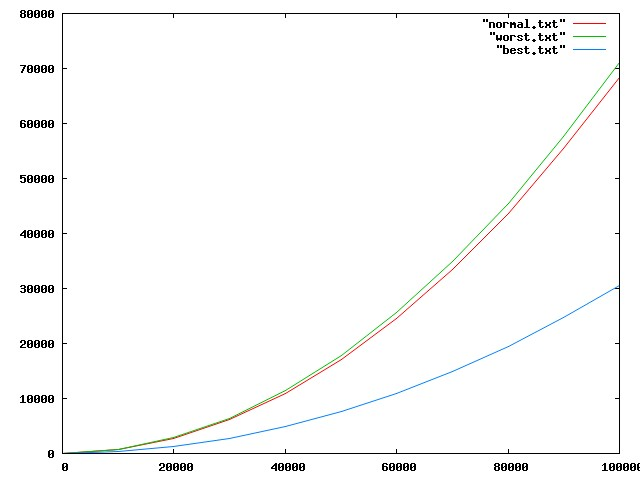
\includegraphics[scale=.5]{bubble.jpg}
\caption{Gnuplot for bubble sort}
\label{fig:bubble}
\end{figure}
\noindent 
Consider test case with numbers -- 4  2  5  1  2 and on each iteration of inner loop,\\ 
  (2  4  5  1  2)$\rightarrow$
  (2  4  5  1  2)$\rightarrow$
  (2  4  1  5  2)$\rightarrow$
  (2  4  1  2  5)$\rightarrow$
  (2  4  1  2  5)$\rightarrow$
  (2  1  4  2  5)$\rightarrow$
  (2  1  2  4  5)$\rightarrow$
  (1  2  2  4  5)$\rightarrow$
  (1  2  2  4  5)$\rightarrow$
  (1  2  2  4  5)


\subsection{Worst Case}
The worst case occurs when the elements are sorted in non-ascending order, because the largest element need to bubbled  till last and hence  the worst case is O(n$^{2}$) time. The graph for worst case is shown in the figure.
\subsection{Best Case}
The best case occurs when the elements are already sorted, because largest element is already in right place and needs no swapping. This case takes O(n) time. The graph for best case is shown in the figure.
\newpage 
\begin{center}
\section{SELECTION SORT}
\end{center}                                                            
\noindent         
Selection sort is one of simplest sorting technique in which we select smallest item in the list and exchange it with the first item.Obtain the second smallest element in the list and exchange it with the second element and so on.Finally all 
the items will be arranged in ascending order.In otherwords selection sort performs sorting by repeatly putting the largest element in the unprocessed portion of the array to the end of the this unprocessed portion until the whole array is sorted.
\newline
\subsection{The Algorithm:}
\begin{tabbing}
\hspace{.5in}\textbf{for} i$\leftarrow$1 to n -- 1\\
\hspace{.75in}\textbf{do} pos $\leftarrow$ i\\
\hspace{.75in}\textbf{for} j $\leftarrow$ i + 1 to n \\
\hspace{1in}\textbf{if} A[j] $<$ A[pos]\\
\hspace{1.25in}\textbf{then} pos$\leftarrow$j\\
\hspace{.75in}\textbf{if} pos $\ne$ i \\
\hspace{1in}\textbf{then} A[i] $\Leftrightarrow$ A[pos]\\

\end{tabbing}
\noindent 
Selection sort has two loops each of which execute \emph{n} times. Hence the selection sort is O(n$^{2}$). The current element is assumed to be the smallest and is compared with remaining elements. The position of the smallest element is found. If the smallest element is not the current position, then the two elements are swapped. \\
  
\begin{figure}[h]
\centering
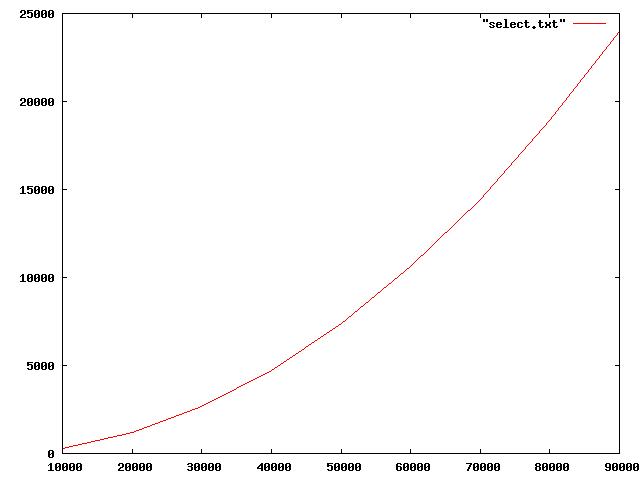
\includegraphics[scale=.6]{select.png}
\caption{Gnuplot for selection sort}
\label{fig:select.png}
\end{figure} 
\noindent 
Consider a test case with elements -- 45 20 40 5 15 \\
(45 20 40 5 15 )$\rightarrow$
(5  20  40  45  15) $\rightarrow$
(5  15  40  45  20)$\rightarrow$\\
(5  15  20  45  40) $\rightarrow$
(5 15 20  40  45) 




\subsection{Worst Case} Worst case occurs if the elements are already sorted in the non-ascending order, because for each iteration the smallest element needs to be swapped and thus the Worst Case is O(n$^{2}$). 

\subsection{Best Case} Best case occurs if the elemsnts are already sorted in non-descending order, because current element is smallest and no element needs to be swapped and thus the Best Case is O(n).\\\\\\\\\\\\\\
\pagebreak 


\begin{center}
\section{THE HEAP SORT}  
\end{center}
This sorting technique builds a max heap tree, in which \emph{none} of the parent nodes are smaller than their children, and then sorts the elements by extracting the topmost element. A sequence of events takes place in this sorting. First the main function calls 'heapSort', which in turn calls buildMaxHeap. This is the basic tool for building the max heap. It builds the max heap tree from the lower nodes to the root by calling the maxHeap function. maxHeap function checks always that parent is larger than their children, and if the property is violated the largest child is exchanged with the parent.\newline

\subsection{The Algorithm:}
\begin{tabbing}
LEFT(i)\\
\hspace{.5in}\textbf{return} 2i + 1\\\\
RIGHT(i)\\
\hspace{.5in}\textbf{return} 2i + 2\\\\
MAX-HEAPIFY(A, i)\\
\hspace{.5in}l $\leftarrow$ LEFT(i)\\
\hspace{.5in}r $\leftarrow$ RIGHT(i)\\
\hspace{.5in}\textbf{if} l $\leq$ \emph{size}[A] and A[l] $>$ A[i]\\
\hspace{.75in}\textbf{then} \emph{largest} $\leftarrow$ l\\
\hspace{.75in}\textbf{else} \emph{largest} $\leftarrow$ i\\
\hspace{.5in}\textbf{if} r $\leq$ \emph{size}[A] and A[r] $>$ A[\emph{largest}]\\
\hspace{.75in}\textbf{then}\emph{largest} $\leftarrow$ r\\
\hspace{.5in}\textbf{if} \emph{largest} $\ne$ i\\
\hspace{.75in}\textbf{then} exchange A[i] $\Leftrightarrow$ A[\emph{largest}]\\
\hspace{1in}MAX-HEAPIFY(A,\emph{largest})
\end{tabbing}
The recurence relation for MAX-HEAPIFY is T(n) $\leq$ T(2n/3) + $\Theta$(1), since each childern's subtrees have a size at most 2n/3 --  the worst case being when the last row of the tree is exactly half full. Thus MAX-HEAPIFY takes T(n) = O(lg n).\newline
\begin{tabbing}
BUILD-MAX-HEAP(A)\\
\hspace{.5in}\textbf{for} i $\leftarrow$ $\lfloor$n/2$\rfloor$ \textbf{downto} 1\\ 
\hspace{.75in}\textbf{do} MAX-HEAPIFY(A,i)
\end{tabbing}
	BUILD-MAX-HEAP takes O(n) time. \pagebreak
\begin{tabbing}
HEAP-SORT(A)\\
\hspace{.5in}BUILD-MAX-HEAP(A)\\
\hspace{.5in}\textbf{for} i $\leftarrow$ n \textbf{downto} 2\\
\hspace{.75in}\textbf{do} exchange A[1] $\Leftrightarrow$ A[i]\\
\hspace{1in}n $\leftarrow$ n -- 1\\
\hspace{1in}MAX-HEAPIFY(A,1)\\
\end{tabbing}
	HEAP-SORT takes O(n lg n) time since call to BUILD-MAX-HEAP takes O(n) time and each of the n--1 calls to MAX-HEAPIFY takes O(lg n) time. \\\\
\noindent 
For the elements - 10, 5, 16, 8, 68, 21, 43; the heapSort procedure results in a non-descendingly sorted elements. The state of the elements at each instance within heapSort iterative with \emph{i} from number of elements to 2 is:\\
\noindent
(10  5 16  8 68 21 43)$\rightarrow$
(16 10 43  8  5 21 68)$\rightarrow$
(16 10 21  8  5 43 68)$\rightarrow$\\
( 5 10 16  8 21 43 68)$\rightarrow$
( 8 10  5 16 21 43 68)$\rightarrow$
( 5  8 10 16 21 43 68)$\rightarrow$\\
( 5  8 10 16 21 43 68) \newline


\begin{figure}[h]
\centering
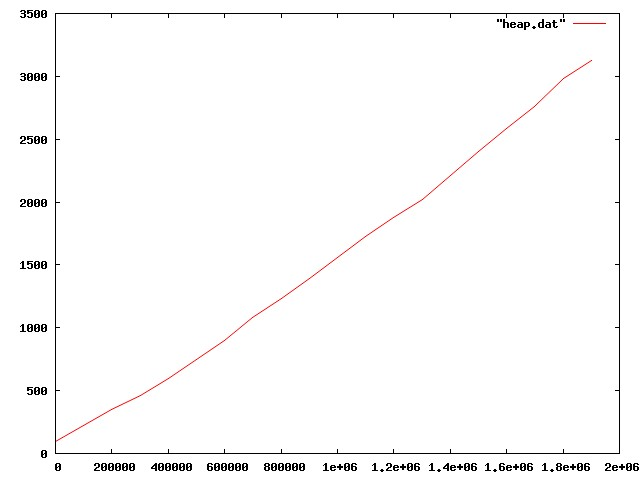
\includegraphics[scale=.45]{heap.jpg}
\caption{GnuPlot for Heap Sort}
\label{fig:heap}
\end{figure}

\subsection{Analysis of Run Times:}
Any of General, Worst or Best Cases of inputs need O(n) time to BUILD-MAX-HEAP. Further, any of "add" or "remove" operations takes O(lg n) time. Hence, runtimes for heap sorting in all the three cases is \emph{always} same with O(n lg n) time.
\newpage

\begin{center}
\section{QUICK SORT}
\end{center}
\noindent 
Quick Sort is based on the technique \emph{'Divide and Conquer'}. It divides the elements into two parts and then sorts them. This sorting is continued recursively till all the elements are sorted. Quick Sort has been implemented using two functions - Partition and QuickSort.\\\\
\noindent 
Paritition routine takes the middle element as \emph{pivot}, rearranging elements such that elements smaller than the pivot is moved onto left of pivot and elements greater than pivot are moved onto its right. This sorting technique swaps the elements even if they are equal, hence is considered as an \emph{unstable algorithm}. \newline 

\begin{tabbing}
PARTITION (A, p, r)\\
	\hspace{.5in}x $\leftarrow$ A[(p + r) / 2]\\
	\hspace{.5in}i $\leftarrow$ p -- 1\\
	\hspace{.5in}j $\leftarrow$ r + 1\\
	\hspace{.5in}\textbf{while} TRUE\\
	\hspace{.75in}\textbf{do repeat} j $\leftarrow$ j -- 1\\
	\hspace{1in}\textbf{until} A[j] $\leq$ x\\
	\hspace{.75in}\textbf{repeat} i $\leftarrow$ i + 1\\
	\hspace{1in}\textbf{until} A[i] $\geq$ x\\
	\hspace{.75in}\textbf{if} i $<$ j\\
	\hspace{1in}\textbf{then} exchange A[i] $\Leftrightarrow$ A[j]\\
	\hspace{1in}\textbf{else return} j
\end{tabbing}
Quick Sort calls the partition subroutine to obtain the pivot element and recursively call itself to sort elements from p$^{th}$  element to pivot and then from pivot to r$^{th}$ element. This recursive call is done until p $<$ r.

\begin{tabbing}
QUICKSORT (A, p, r)\\
	\hspace{.5in}\textbf{if} p $<$ r\\
	\hspace{.75in}\textbf{then} q $\leftarrow$ PARTITION(A, p, r)\\
	\hspace{1in}QUICKSORT(A, p, q)\\
	\hspace{1in}QUICKSORT(A, q+1, r)
\end{tabbing}

The steps for sorting of an input is given below :-\\
\noindent (4 2 3 5 1)$\rightarrow$
(1 2 3 5 4)$\rightarrow$
(1 2 3 5 4)$\rightarrow$
(1 2 3 5 4)$\rightarrow$
(1 2 3 5 4)$\rightarrow$
(1 2 3 5 4)$\rightarrow$
(1 2 3 5 4)$\rightarrow$
(1 2 3 4 5)$\rightarrow$
(1 2 3 4 5)$\rightarrow$
(1 2 3 4 5)$\rightarrow$
(1 2 3 4 5)

\subsection{Worst Case}
The Worst case happens when the elements are already sorted. The partition routine returns the value as i+1. Thus the quicksort has to call partition n times and there is a loop of n times inside the partition.Thus the order of the quickSort becomes \\
T(N) = T(N-1) + O(N)\newline 
T(N) = O(N$^{2}$) \newline

\begin{figure}[h]
\centering
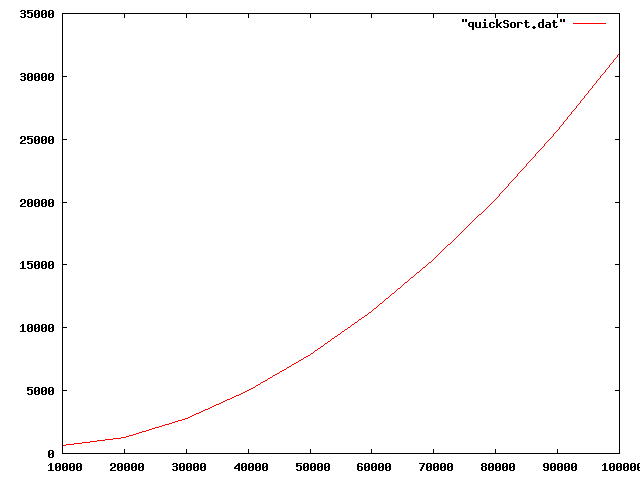
\includegraphics[scale=.5]{qworst.png}
\caption{Plot for Quick Sort Worst Case}
\label{fig:qworst}
\end{figure} 

\subsection{Best Case}

The Best case is when the partiton function returns the middle element. when this happens, the array is split into half and N reduces by half every time. Thus in the best case, We get the time of QuickSort as \\
T(N) =  $\leq$ 2T(n/2) + O(n)
T(N) = O(n lg n) 
\begin{figure}[h] 
\centering
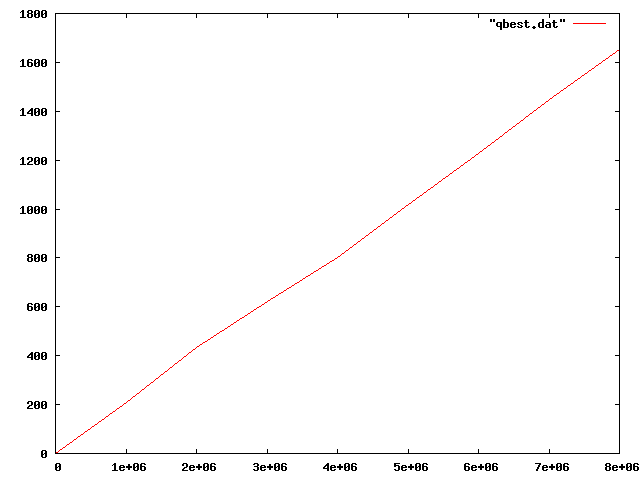
\includegraphics[height=2.5in]{qbest.png}
\caption{Plot for Quick Sort Best Case}
\label{fig:qbest}
\end{figure} 
\noindent
\pagebreak
\begin{figure}[h] 
\centering
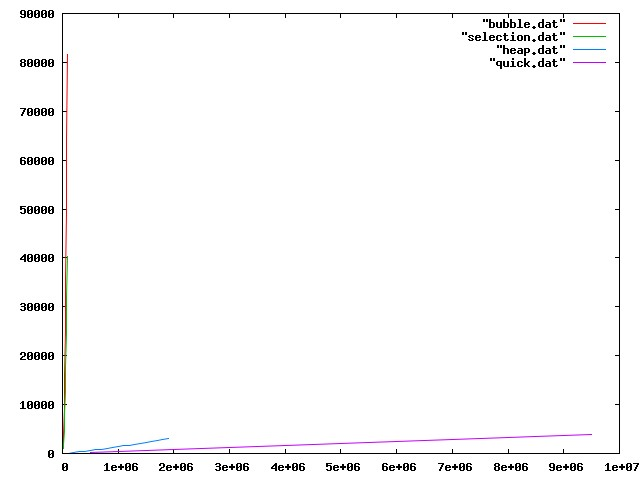
\includegraphics[height=2in,width=5in]{comparision.jpg}
\caption{Comparing All Sorts}
\label{fig:compare}
\end{figure} 

Comparing all the sorts---Bubble, Selection, Heap and Quick, there was huge difference in order of time.\\\\\\\\\\\\\\\\
\newpage 
\begin{thebibliography}{99}
\bibitem{} Cormen, Thomas H et al, 2005, \emph{Introduction to Algorithms---Second Edition}, Prentice-Hall of India.
\bibitem{} Levitin, Anany, 2003, \emph{Introduction to The Design $\&$ Analysis of Algorithms}, Pearson Education 
\\\\ \textbf{\LaTeX\ References} \\
\bibitem{} LESLIE LAMPORT, 1985, \emph{\LaTeX---A Document Preparation System---User's Guide And Reference Manual},Addison-Wesley, Reading.
\bibitem{} \LaTeX\ Tutorials, 2003, \emph{A Primer---Indian \TeX\ Users Group}, India.
\bibitem{} Greenberg, Harvey J, 1999, \emph{A Simplified Introduction to \LaTeX\ }, Denver.
\bibitem{} \emph{Internet Sources} 
\end{thebibliography}



\end{document}
